\documentclass[11pt]{article}
\usepackage{common,graphicx,subfig,hyperref}

\pagenumbering{roman}
\title{CS182 Artificial Intelligence Project \\ \Large{Safe Cycling Route Planning}}
\author{Anna Sophie Hilgard, Nick Hoernle, and Nikhila Ravi}
\begin{document}
\maketitle{}

% % Some new environments for fancy cross-referencing
% \newenvironment{a_star_algorithm}[1][htb]
%   {\renewcommand{\algorithmcfname}{$A^{*} Star Algorithm$}% Update algorithm name
%    \begin{algorithm}[#1]
%   }{\end{algorithm}}


\setlength{\parindent}{2em}
\setlength{\parskip}{1em}
\renewcommand{\baselinestretch}{1.3}
\pagenumbering{arabic}

\section{Introduction}

Biker safety and biker safety awareness has been a topical issue for a number of years with the biker death toll at an unacceptably high rate (13 deaths in the past 5 years in Boston alone and 876 recorded accidents involving bikes and cars in Cambridge in the past 5 years. Current mapping applications like Google maps often route cyclists through busy streets and intersections, resulting in unnecessarily dangerous trips. The purpose of this project has been to explore AI graph search and local search algorithms to optimize a bike routing algorithm not only for `distance minimization', but also for `path safety' and `elevation comfort'. We explore the use of $A^{*}$ graph search under different cost and heuristic metrics to obtain a fast, yet reliable graph search between any two nodes on the intersection graph. Furthermore, we explore the use of local search to optimize for the ideal meeting point between two or more cyclists.

% \par The algorithm we chose to use for this problem is $A^{*}$ search with a variety of cost functions and heuristics incorporating distance, safety of a given route, and changes in elevation (also important for biking but not information Google maps currently considers).

% \par The graph search problem is directly analogous to techniques and ideas from the class: using intersections as nodes in the graph and road segments connecting intersections as paths, we are able to construct the city maps as directed graphs. From there, we can use data generated from a variety of sources to come up with approximate costs associated with paths and related heuristics at nodes.

% \par The optimization techniques we use are also direct applications of algorithms from the optimization portion of the course.

% Problem-specific adaptations were largely limited to the collection and interpretation of relevant data and the development of a cost function and relevant heuristics.

\section{Background and Related Work}

While our problem was fairly straightforward, we did do some research to get ideas for potential cost attributes and data sources. Our initial formulation of the problem, for example, did not include elevation differencing, but reading previous studies led us to believe that this was an important criterion \cite{pmbr}.

\section{Problem Specification}
The graph of intersections and nodes forms a highly connected state space (Cambridge has 1831 nodes, San Francisco has 18410 nodes, and each node typically has a branching factor of 4). While it is possible, searching the entire state space for San Francisco would involve considerable computation, on the order of $4^{18410}$ possible routes to explore, and this search space grows exponentially with additional nodes.
\par To compound this search space problem, we aimed to determine central meeting areas for a number of cyclists to use as a fair and safe meeting place. The search problem here is therefore not only to determine the best route from a start node to a goal but also to determine the best goal node, optimizing for minimal cost for all cyclists.
\par Initially, we implement an $A^{*}$ search algorithm. We then used that $A^{*}$ search as a baseline for determining the route from any starting point to some goal node and we run a local search layer on top of this to find the best meeting intersection between a number of cyclists. We tailored three cost functions and three heuristics for comparing the performance of the $A^{*}$ and Local Search (which depend on the $A^{*}$ algorithm).

\subsection{Cost Functions}
We seek to minimize some cost function:
\begin{equation}
cost = \sum_{i=0}^n cost(path_i)
\end{equation}
given that:
\begin{itemize}
\item $path_0 \in Connections_{\text{(starting node)}}$
\item $path_i, path_{i+1} \in Connections_{node_i}$
% \item $path_i, path_{i-1} \in Connections_{node_k}$
\item $path_n \in Connections_{\text{(target node - 1)}}$
\end{itemize}

\noindent Specifically for our problem, we created three different cost functions:
\begin{align}\label{cost_fns}
cost_{distance\_only}(path_i) &= length_i \\
cost_{distance\_safety}(path_i) &= (\alpha \times length_i) \times  (\beta \times accidents_i) \\
cost_{distance\_safety\_elevation}(path_i) &= (\alpha \times length_i) \times  (\beta \times accidents_i) + abs(\Delta elevation_i)
\end{align}


\noindent Where $\alpha$ and $\beta$ are scaling multipliers to weight the relative magnitudes of the different cost measurements. We used a value of $\alpha = 10000$ to scale the coordinate based length measurement to a number on the same magnitude of $\Delta elevation$. $\beta$ was set to 5 to penalize the roads with accidents highly in the algorithm. These values can be tuned empirically.\par
\noindent In the optimization portion of our project, we seek to minimize the total cost to all parties:
\begin{equation}
min(\sum_j^n cost_j)
\end{equation}
where $cost_j$ is the cost to participant j.

\section{Approach}
\subsection{Data Structures}
Our primary data structures are an intersection graph, which is stored as a Python dictionary, and a connection dictionary, which is also stored as a Python dictionary. The intersection graph maps nodes (intersections) by id to a list of paths (road segments) from that node. The connection dictionary maps a connection (road segment) to its source node, sink node, and various cost parameters (in our case distance, number of bicycle crashes on that road segment, and change in elevation over that road segment).

\subsection{Data Collection, Extraction and Preprocessing}
In this case study, we were able to use open source geolocation data from Cambridge and San Francisco city councils. These departments further supplied data on the number of bike related accidents for various road segments. Lastly an elevation layer from the open GIS websites was used to infer the elevation of certain roads and intersections.

We tested our implementation on data from the cities of Cambridge, MA and San Francisco, CA. GIS location data is available on the local government websites in the form of a pandas geojson dataframe and was easily read into a pandas dataframe object using the geopandas library \footnote{\url{http://geopandas.org/}}.
\par
As discussed above, these geolocation data are used to create a set of nodes with coordinate positions and a number of connections which define the roads and the intersections that those roads are connected to. The data from Cambridge contained routing errors where some intersections were connected to other incorrect intersections resulting in roads that spanned the entire graph rather than simply connecting the two nearest neighboring intersections. The solution to this was to use the $geometry$ data within the Pandas geolocation dataframe and the $shapely$ \footnote{https://pypi.python.org/pypi/Shapely} graphing library to compare the actual road length to our interpolated distance for the road. If the interpolated distance was incorrect by more than a factor of 10, we made the assumption that the nodes were incorrectly tagged in the data and we therefore dropped the connection attribute. The elevation and crash data was independently collected from the different government websites and the intersection id's were used to map this data into the `intersection' and `connection' graphs and dictionaries.
\par The resulting connected graphs for `Cambridge' and `San Francisco' are shown in figure \ref{connected_graphs}

\begin{figure}%
    \centering
    \subfloat[San Francisco]{{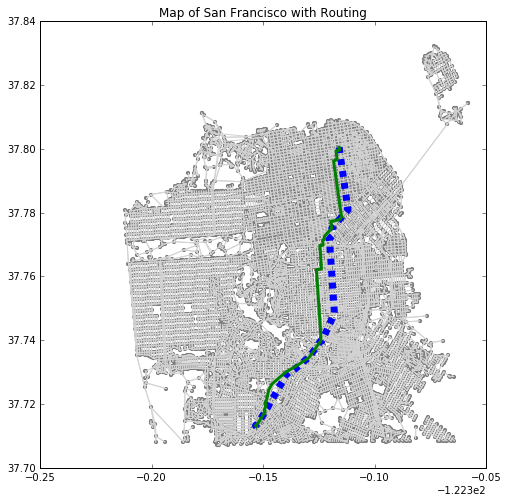
\includegraphics[width=7cm]{../images/san_fran_map} }}%
    \qquad
    \subfloat[Cambridge]{{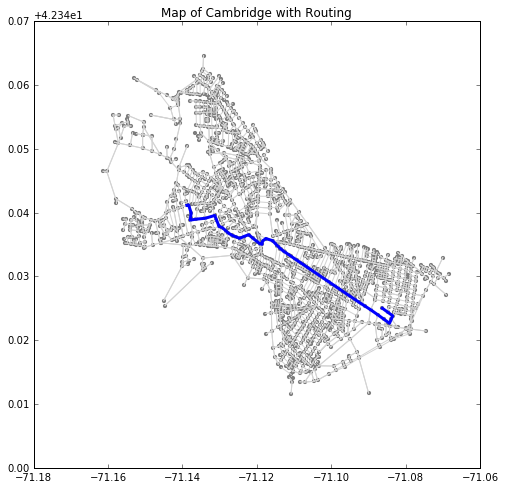
\includegraphics[width=7cm]{../images/cambridge_map} }}%
    \caption{Connected graphs of the San Francisco and Cambridge maps with a route shown on the map (using only distance as the cost metric on the Cambridge but distance and safety on the San Francisco map).}
    \label{connected_graphs}%
\end{figure}

\subsection{$A^{*}$ Search}
$A^{*}$ is an adaptive graph search algorithm that is able to take different cost and heuristic functions as parameters and then traverses the graph based on the output of these functions. $A^{*}$ search was chosen over the uniform cost alternative due to the efficient graph search under a good heuristic. We note that while a simple heuristic is to use the Euclidean distance to the goal node, incorporating accident and elevation data is non-trivial and may lead to inconsistent heuristic functions.\par
Please refer to Appendix \ref{algorithms}, \nameref{a_star_algo} for a formal outline of the algorithm.

\subsubsection{Heuristic Functions}
We used three main heuristic functions for testing the $A^{*}$ algorithm. We firstly used a null heuristic that we use as a baseline to compare the other heuristics against. We used a simple euclidean distance heuristic that measures the distance from the current node i to the goal node as an admissible and consistent heuristic. Finally we used a heuristic that makes a simple delta elevation estimate from the current goal to the end goal and a minimum of the number of accidents on the connections from the current goal. This `combined heuristic' also included the euclidean distance element and a linear combination of these values was used.
\begin{align}\label{heuristic_fns}
heuristic_{null}(node_i) &= 0 \\
heuristic_{euclidean\_distance}(node_i) &= euclidean\_distance(node_i, goal)\\
\begin{split}
heuristic_{combined}(node_i) &= (\alpha \times euclidean\_distance(node_i, goal) \\ &\times  (\beta \times min(accidents\_node_i)) \\&+ abs(elevation\_difference(node_i, goal))
\end{split}
\end{align}

\subsection{Local Search: Simulated Annealing}
The Simulated Annealing Search involved initializing a centroid and iteratively hill climbing the space around that centroid to find a local optimum point. Initially, a temperature attribute is set high, such that the hill climbing algorithm accepts non-optimal nodes with a high probability. As the algorithm proceeds, and converges on a local optimum, the temperature is decreased such that the hill climbing becomes more deterministic.
\par
As the state space of the search graph is large, and the distance metric is highly interpretable, we opted to initialize the first centroid at the intersection that represents the Euclidean mean between all cyclists. Our aim was to initialize the centroid within the vicinity of an optimal meeting point and allow the high initial temperature to counteract any potential local optimum intersections that may have been encountered.
\par
Please refer to Appendix \ref{algorithms}, \nameref{annealing_algo} for a formal outline of the algorithm.

\subsection{Local Search: K-Beam Search}

K Beam search involved initializing a number of centroids within the state space of the graph and iteratively hill climbing from the K best centroids to find a local optimum.
\par
Please refer to Appendix \ref{algorithms}, \nameref{k_beam_algo} for a formal outline of the algorithm.

\section{Experiments}
% Analysis, evaluation, and critique of the algorithm and your
% implementation. Include a description of the testing data you used and
% a discussion of examples that illustrate major features of your
% system. Testing is a critical part of system construction, and the
% scope of your testing will be an important component in our
% evaluation. Discuss what you learned from the implementation.
We aimed to test:
\begin{itemize}
\item The effect of the varying cost functions on the routes that were found.
\item The effect of the $A^{*}$ heuristic on the speed of search (and consistency of the route)
\item The efficiency and effectiveness of the resulting search
\end{itemize}

\subsection{Testing $A^{*}$ Search}
We randomly selected nodes within the two graphs and ran $A^{*}$ search to find the optimal route through the map. The figure \ref{fig:connected_san_fran} shows an example of $A^{*}$ finding an optimal route under two different costs.

\begin{figure}
\center
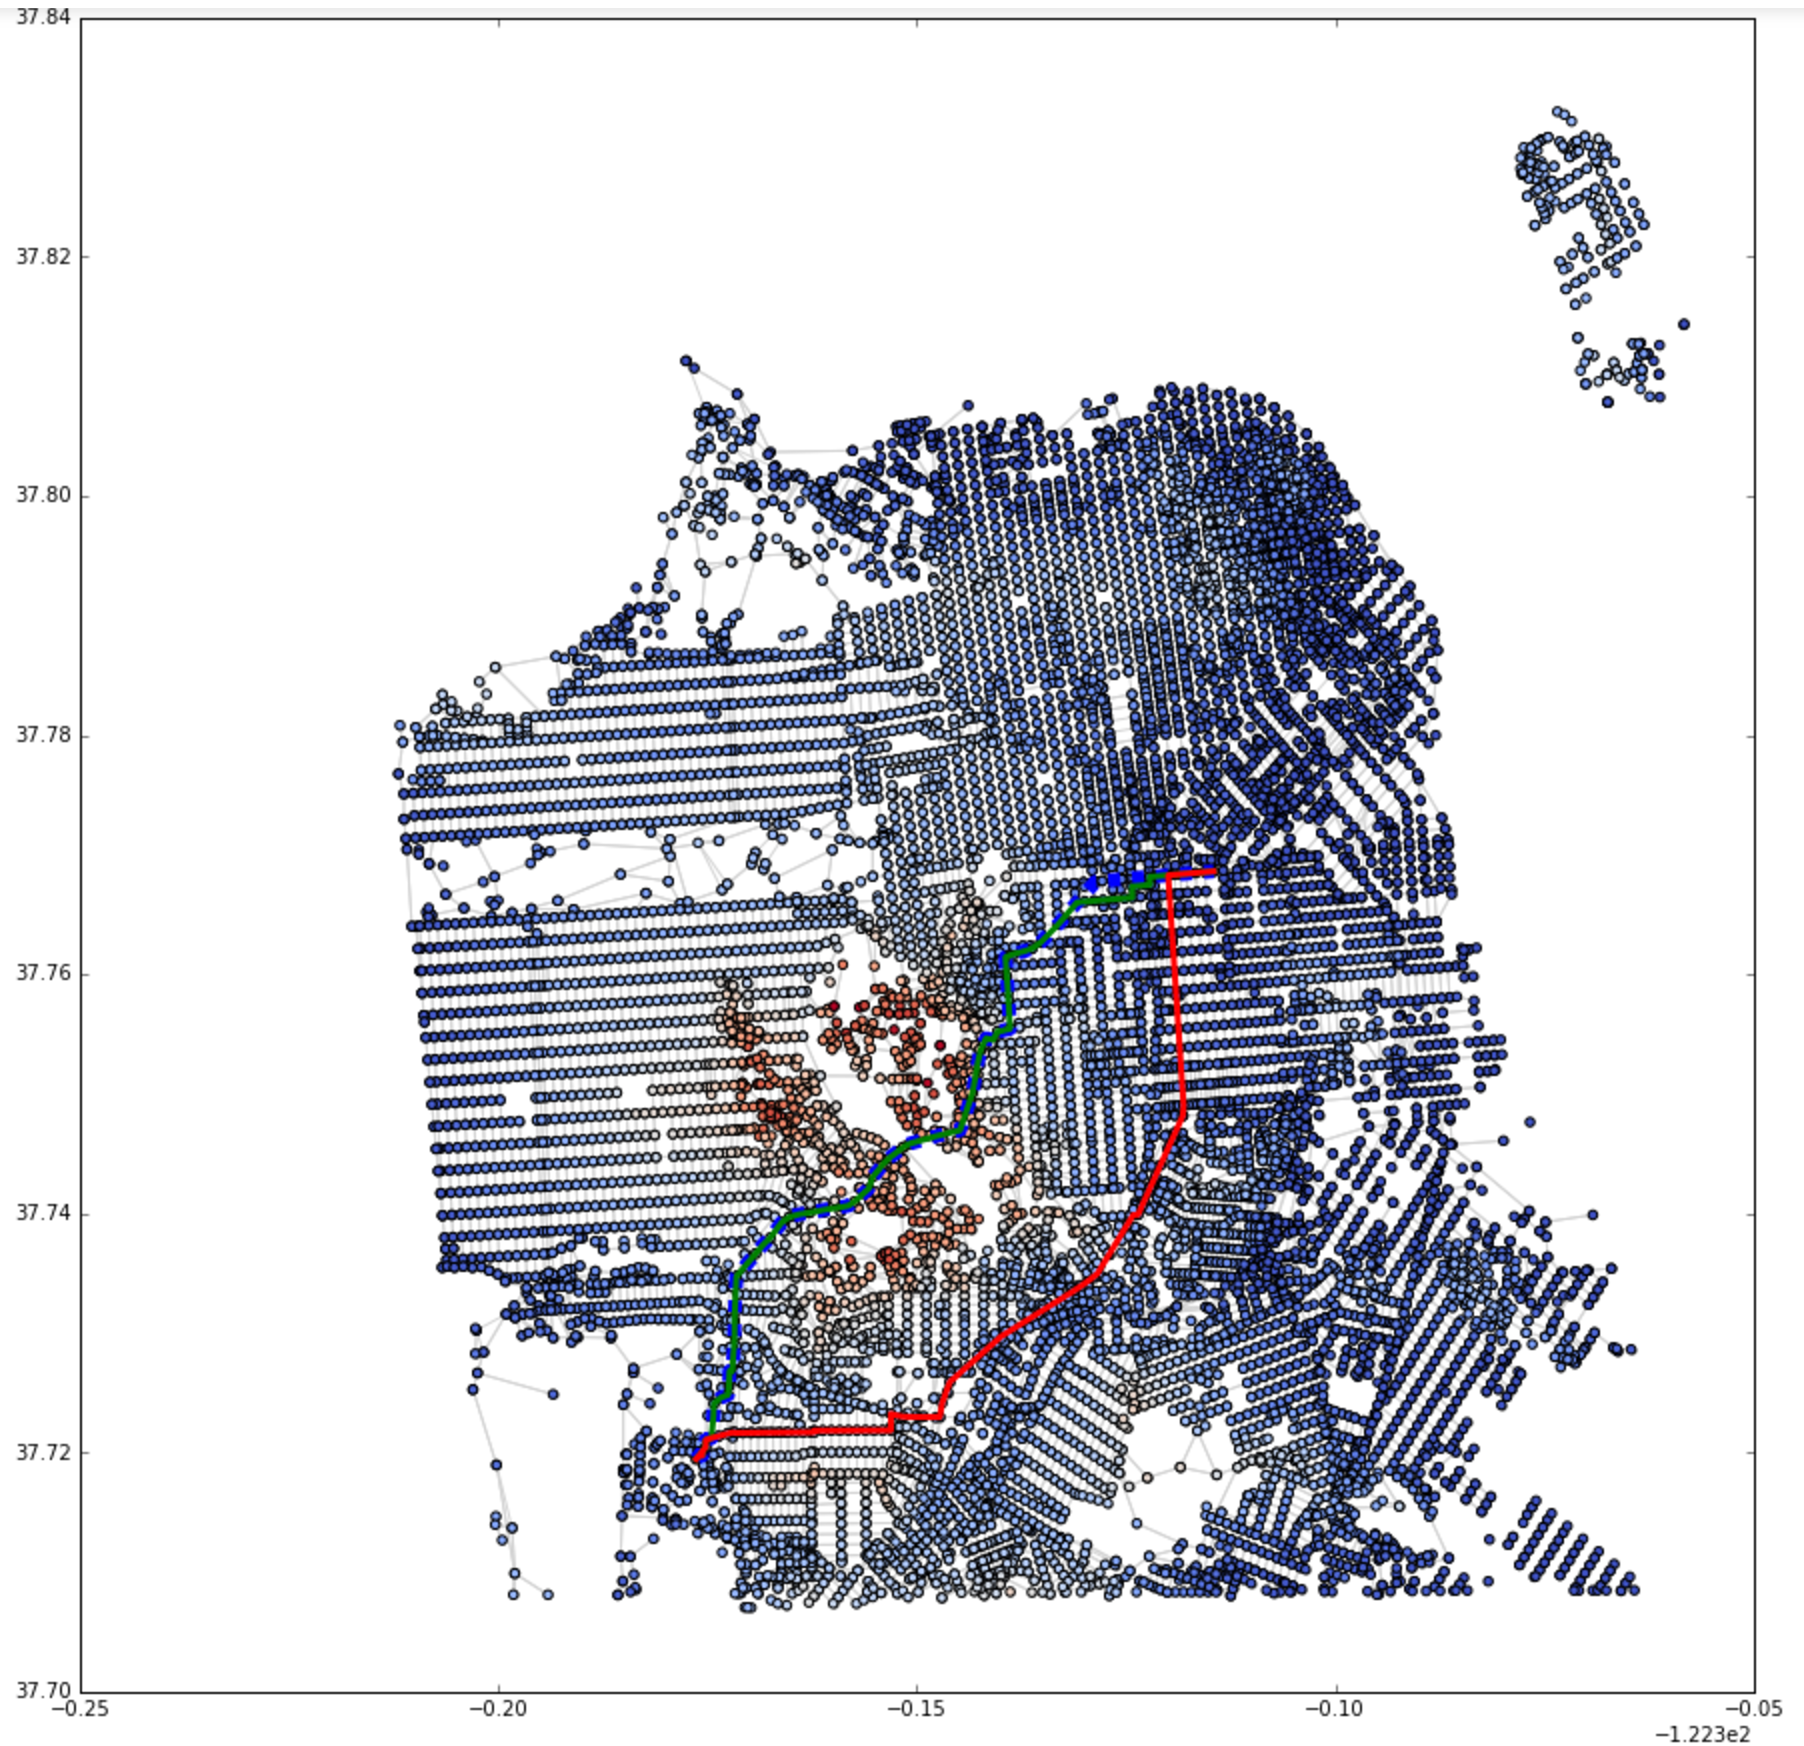
\includegraphics[width=0.6\textwidth]{../images/sf_new_plot_2.png}
\caption{Paths between nodes in San Francisco. Blue path optimizes for distance only, green path avoids previous bicycle accidents, and red path minimizes altitude changes. Overlaid with an altitude plot of San Francisco, we can clearly see the red path avoiding a hill.}
\label{fig:connected_san_fran}
\end{figure}

\par
We then ran an iteration of 100 simulations for each cost function (\ref{cost_fns}) and each heuristic function (\ref{heuristic_fns}). Specifically the null and euclidean heuristics are both expected to find the optimal route. The euclidean heuristic should explore fewer nodes than the null heuristic. When the cost function is simple distance or simple distance and safety, the combined heuristic is neither admissible nor consistent as it is penalizing nodes for a cost that is not encoded in the algorithm. We expect to see this algorithm find a `longer than necessary optimal path'. However, when the cost function also encodes all of these costs, we now expect the combined heuristic to out perform the other heuristics on all accounts. Please refer to \nameref{results} for a further discussion on the above.

\subsection{Testing Local Search}

We ran Simulated Annealing and K-Beam Search on a number of different iterations of randomly selected nodes. While both algorithms can be tuned to run faster (by reducing the temperature faster for simulated annealing and reducing `k' for k-beam search at the cost of being more susceptible to local minima) we can make a reasonable comparison of the two algorithms in terms of their total runtime and resulting cost of the returned node.

\section{Results}\label{results}

\subsection{$A^{*}$ Search Results}
Initially we ran a test of the different cost functions using a null heuristic. We are thus guaranteed to find the optimal solution for each of the cost functions (this is analogous to uniform cost search) but this search is inefficient. For this experiment, we are interested in comparing the cost functions and thus this is not important.
\par

Figure \ref{cost_comparison} shows the route distance, number of nodes searched and the total change in elevation of the route vs the euclidean distance from source node to goal node for different routes, changing the cost function that is used in the $A^{*}$ search. Here we see that the basic road cost will find the shortest possible route to the solution, but as additional costs are added to certain road segments the distance of the other solutions will increase. Interestingly, the three cost functions often require the same number of nodes to be searched. Lastly, we see that the combined cost function generally results in a solution that has the lowest total change in elevation (the uncommon event when it does not result in the lowest elevation is because it is also optimizing over the distance and the number of accidents on each road link).

\begin{figure}[H]
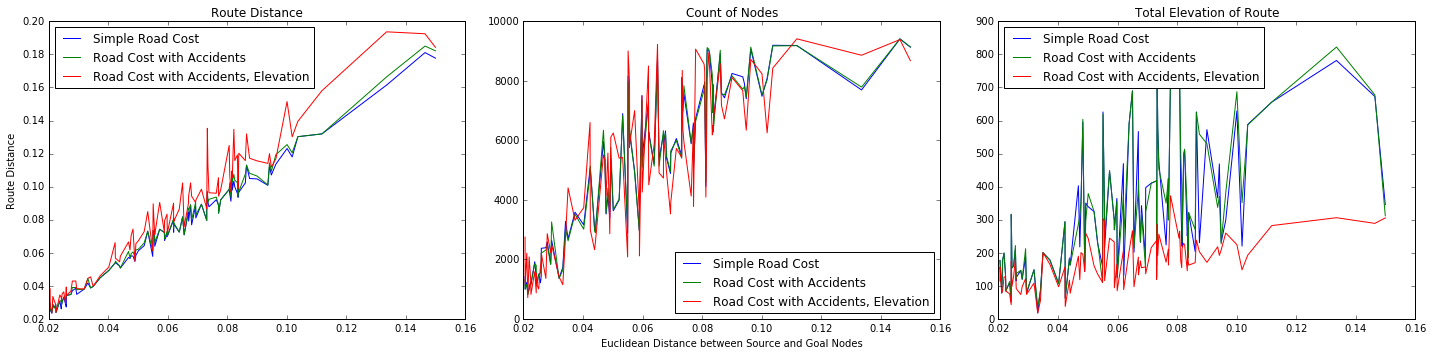
\includegraphics[width=1\textwidth]{../images/cost}
\caption{Basic metrics for the three cost functions.}
\label{cost_comparison}
\end{figure}

In Figure \ref{simple_distance_cost} we see that the combined heuristic significantly under performs the null heuristic and euclidean heuristic in terms of distance as the heuristic does not properly model the cost function (it is adding expected costs for each node that do not actually exist). This heuristic is therefore not admissible for these cost functions and it does not return the optimal path to the solution. The euclidean heuristic still finds the optimal path but it expands far fewer nodes than the null heuristic.

\begin{figure}[H]
\caption{Varying the three heuristics for the basic road distance cost.}
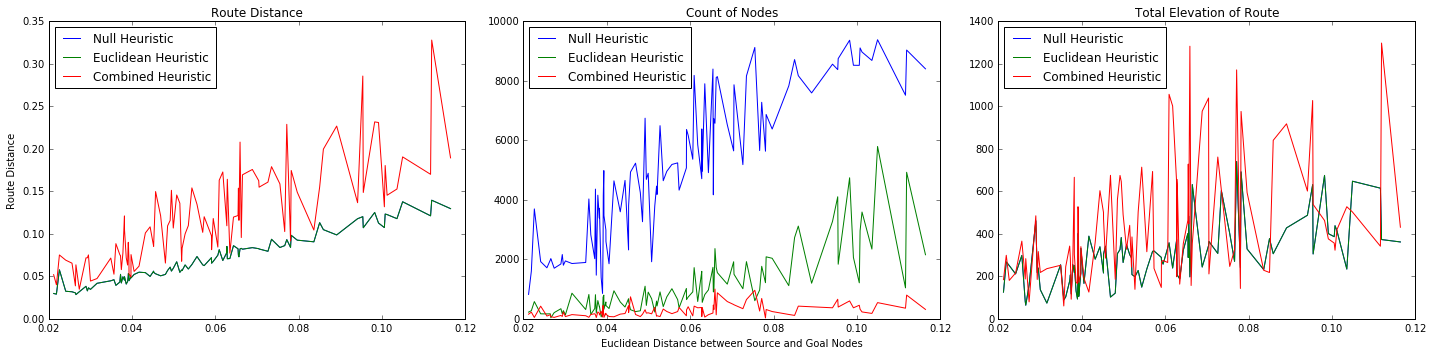
\includegraphics[width=1\textwidth]{../images/simple_distance_cost}
\label{simple_distance_cost}
\end{figure}

Again, figure \ref{simple_distance_and_safety} shows that the combined heuristic is not admissible. The euclidean heuristic again far outperforms the null heuristic in terms of nodes searched.

\begin{figure}[H]
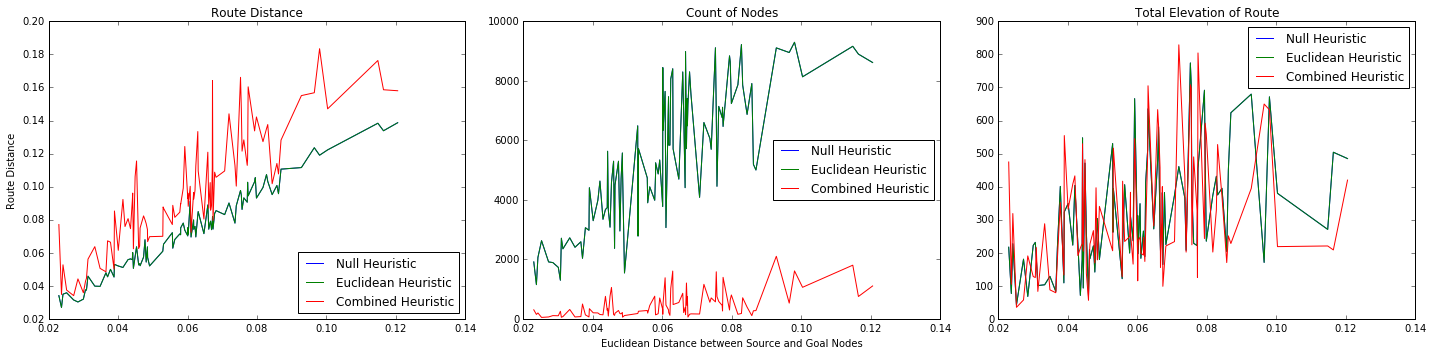
\includegraphics[width=1\textwidth]{../images/simple_distance_and_elevation}
\caption{Safety road cost under three different heuristics.}
\label{simple_distance_and_safety}
\end{figure}

Finally, we see in \ref{simple_distance_elevation_and_safety} that the the combined heuristic returns a path that is comparable to the other two heuristics (in terms of path distance). The fact that it is different suggests that the heuristic might not be admissible as the number of accidents from one node to the next may be dramatically different from what the heuristic is guessing (this is a very hard parameter to model). However, the fact that this heuristic now does model the accident and elevation costs that are present means that it is very efficient in finding an optimal route (in terms of numbers of nodes searched).

\begin{figure}[H]
\caption{Safety, distance, and elevation cost under three different heuristics.}
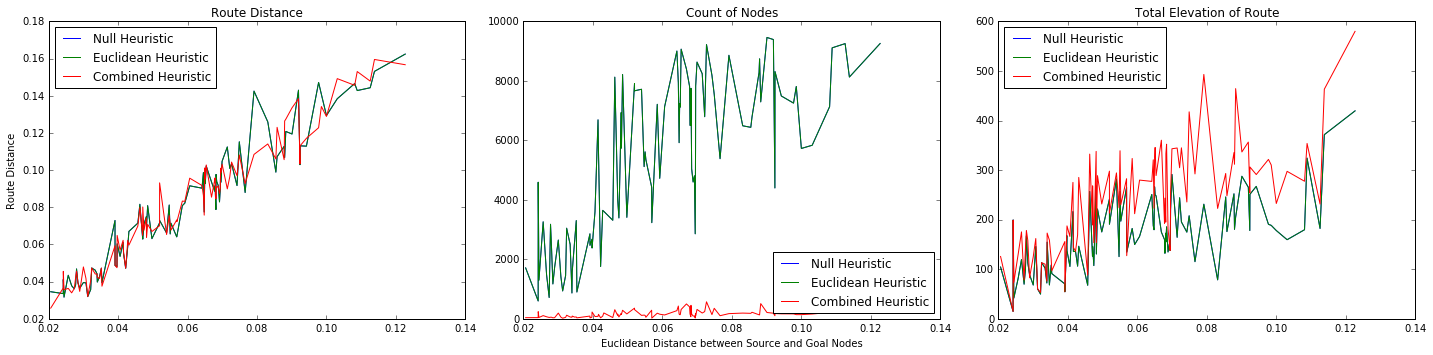
\includegraphics[width=1\textwidth]{../images/simple_distance_elevation_and_safety.png}
\label{simple_distance_elevation_and_safety}
\end{figure}

\subsection{Local Search Results}
As for the $A^{*}$ search evaluation, we randomly selected 4 nodes and computed the time that it took the algorithm to converge and the overall cost of all routes to the final returned centroid location. In figure \ref{sim_ann_and_k_beam_cost} we see that k beam generally finds a solution centroid with a slightly lower cost than simulated annealing. Furthermore, from \ref{sim_ann_and_k_beam_time}, apart from under the null heuristic, we see that k beam search with $k=5$ has a very comparable search time to that of simulated annealing.

\begin{figure}[H]
\center
\caption{Time to compute the centroid node for both Simulated Annealing and K Beam search (with $k = 5$)}
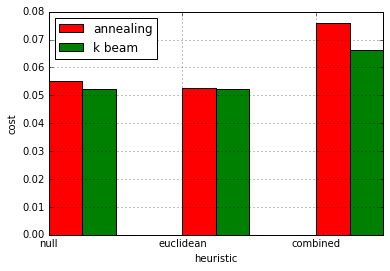
\includegraphics[width=0.6\textwidth]{../images/sim_ann_and_k_beam.png}
\label{sim_ann_and_k_beam_cost}
\end{figure}

\begin{figure}[H]
\center
\caption{Total cost of routes from all starting nodes to the returned centroid for both Simulated Annealing and K Beam search (with $k = 5$)}
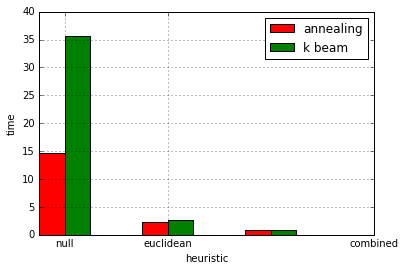
\includegraphics[width=0.6\textwidth]{../images/sim_ann_and_k_beam_time.png}
\label{sim_ann_and_k_beam_time}
\end{figure}

The reason for k beam search out performing simulated annealing is the presence of very definite local optima. The initialization of multiple random start points within a reasonable area of possibilities has a greater chance of initializing close to the solution than the simulated annealing. Even with the temperature set at a high value, the simulated annealing struggles to fully leave the vicinity of the node that it is initialized at (and since this is deterministically the absolute center of all the cyclists, especially if the route is hilly or has many road accidents, it may be far from the global optimum point).
\par
While the k beam solution does out perform the simulated annealing solution, in practice we do see that the costs are still comparable and thus the solution that the simulated annealing returns is still valid. The below figure \ref{overall_plot} is a plot showing the centroid found between four cyclists (under the combined cost cost function and combined heuristic).

\begin{figure}[H]
\caption{Plot showing the centroid found between four cyclists in Cambridge, and each cyclist's route to the solution. The plot encodes the cost of every other node in the map as if it were the solution (and thus shows the high cost nodes in red - i.e. unlikely centroids) and the low cost nodes in yellow (i.e. likely centroids). We further see from this plot that while the combined cost for the four cyclists is not necessarily the same as the cost of only one cyclist, the route that the $A^{*}$ algorithm finds generally follows a path that avoids the red high cost nodes.}
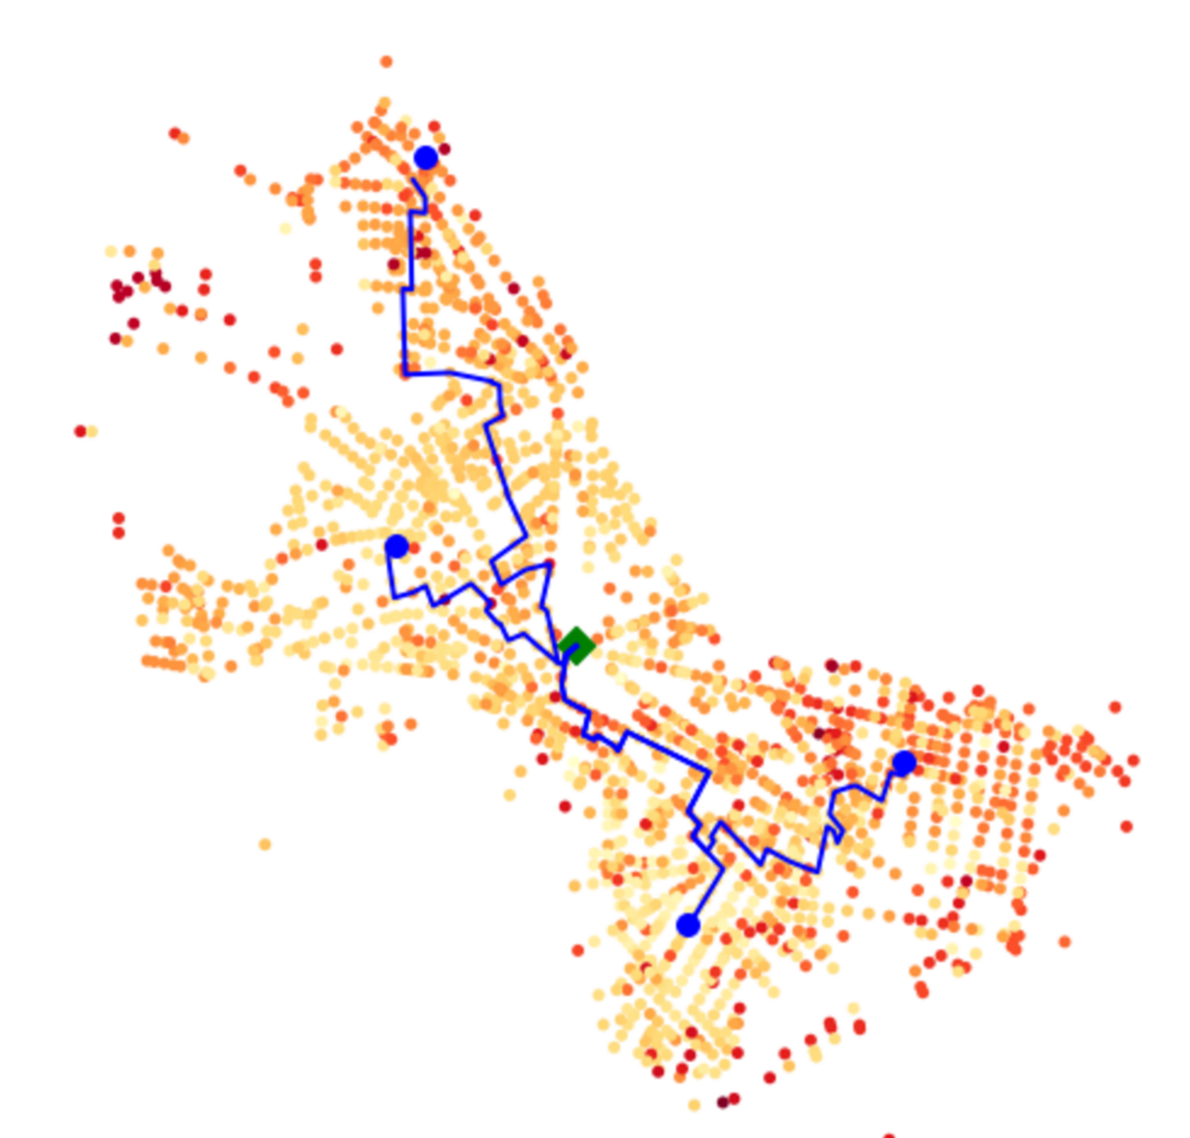
\includegraphics[width=1\textwidth]{../images/overall_plot.png}
\label{overall_plot}
\end{figure}

\section{Discussion}

Our algorithms could have been made to run somewhat faster by incorporating pruning strategies but we were generally satisfied with run times (especially when evaluating the combined heuristic with the distance, safety and elevation costs). Additionally, it was difficult to generate a very useful admissible heuristic for bike crashes because one could almost always find an extremely convoluted path to avoid almost all of them, and so to have a heuristic which is always $\le$ the actual cost to the goal is often not consistent. However, even without being consistent (i.e. it was returning a solution that was slightly different from the optimal solution), the heuristic did provide a very good solution for the problem.
\par
Furthermore, calculating the number of accidents per road segment is a good estimate of how dangerous a given road segment is, but probably a better indicator would be accidents per units of bicycle traffic. If we were able to collect bicycle traffic data for each road segment, we could then calculate the Bayesian probability of:
\begin{equation}
P(\text{road segment | accident}) \propto P(\text{accident | road segment}) * P(\text{road segment})
\end{equation}In particular, we may be over-penalizing roads with a large amount of cycling traffic.
\par
The graph search approach shows a very feasible solution to this problem of intelligent routing. We felt that our results were very reasonable given our preexisting knowledge of Cambridge and San Francisco streets.
\par
\noindent Takeaways from this project:
\begin{itemize}
\item You're only as good as your data. We had some lofty goals for the data that we'd be able to collect and use for this project, but even the data we ended up using was harder to collect and map than we had originally anticipated. Furthermore, while still applicable to testing these algorithm implementations, much of the crash data was a few years old and thus to be more applicable we would want to include a real time update to the data and an expiration of old data. Cambridge and San Francisco are relatively tech-forward cities, so we can imagine this would be even more difficult in most other environments.
\item We initially built the system for the Cambridge data but then obtained the larger mapping data for San Francisco. It was therefore interesting to see how our algorithm scaled to the larger map of San Francisco. To plan routes through a larger area, it's clear that we would have to adapt the algorithm to get the runtime within a reasonable range. In particular, we found in our reading that many routing engines actually use inadmissible heuristics for these tasks and still find reasonable results but in a much quicker time.
\end{itemize}

\newpage
\appendix
\section{System Description}

The easiest way to use our system is to open the provided iPython notebook and run each of the cells. All of the supporting functions can be found in $final\_project.py$.\footnote{$final\_project.py$: \url{https://github.com/NickHoernle/Artificial-Intelligence-CS182-Project/blob/master/final_project.py}} \footnote{$final\_project.ipynb$: \url{https://github.com/NickHoernle/Artificial-Intelligence-CS182-Project/blob/master/final_project.ipynb}}

\section{Group Makeup}

\begin{enumerate}
\item Nicholas Hoernle
\begin{enumerate}
\item Creation of graph dictionary structure and $A^{*}$search algorithm
\item Simulated annealing
\end{enumerate}
\item Nikhila Ravi
\begin{enumerate}
\item K-Beam Search
\item Visualization and analysis of results of graph search algorithms
\end{enumerate}
\item Anna Sophie Hilgard
\begin{enumerate}
\item Construction of Datasets
\item Research and Implementation of more complicated cost functions and heuristics
\end{enumerate}
\end{enumerate}

\section{Algorithms}\label{algorithms}
\begin{algorithm}[H]
  \caption{$A^{*}$ Search Algorithm}\label{a_star_algo}
  \begin{algorithmic}
    \Function{A-Star-Search}{$graph, start node, target node$}
    \State{$node \gets $a node with $ \textsc{state}=start node$}
    \State{$\textsc{path-cost} \gets \textbf{heuristic}(start node, target node)$}
    \State{$frontier\gets $ a priority queue ordered by $\textsc{path-cost} + \textbf{heuristic}(node, target node)$ with $node$ as the only element}
    \State{$explored \gets $ an empty set}
    \Loop
    \If{$\textsc{Empty?}(frontier)$}
    \State \textbf{return failure}
    \EndIf
    \State{$node \gets \textsc{pop}(frontier)$ /*chooses the lowest cost+heuristic node in $frontier$ */}
     \If{$node == targetnode$}
    \State {\textbf{return} \textsc{solution}($node$)}
    \EndIf
    \State{add node.\textsc{State} to $explored$}
    \For{ \textbf{each} $path$ in \textsc{Paths}($node$)}
    \State{$child \gets$ \textbf{child-node}($node, path$)}
    \If {$child$.\textsc{State} is not in $explored$ or $frontier$}
    \State{$frontier \gets$ \textbf{insert}($child, frontier$)}
    \ElsIf  {$child$.\textsc{State} is in $frontier$ with higher \textsc{path-cost} + heuristic}
    \State{replace that $frontier$ node with $child$}
    \EndIf
    \EndFor
    \EndLoop
    \EndFunction{}
  \end{algorithmic}
  \caption{A-Star Search}
\end{algorithm}

\begin{algorithm}[H]
  \caption{Simulated Annealing Algorithm}\label{annealing_algo}
  \begin{algorithmic}
    \Function{Simulated Annealing Meeting Spot}{$graph, startingpts, cost, heuristic$}
    \If{$\textbf{length}(startingpts)<2$}
    \State \textbf{return error}
    \EndIf
    \State{$current \gets$ \textbf{mean}$(startingpts)$.\textsc{closest-node}}
    \State{$temperature \gets e^{10}$}
    \State{$\gamma \gets .5$ /*schedule to manage $temperature$ */}
    \While{$temperature > e^{-2}$}
      \State{$temperature \gets temperature*\gamma$}
      \State{$next \gets$ a randomly selected $child$ of $current$}
      \State{$current.\textsc{value} \gets \sum_{pt \in startingpts}\textbf{cost}(pt, centroid$)}
      \State{$next.\textsc{value} \gets \sum_{pt \in startingpts}\textbf{cost}(pt, next$)}
      \State{$\Delta E \gets next.\textsc{value} - current.\textsc{value}$}
      \If {$\Delta E > 0$}
      \State{$current \gets next$}
      \Else
       \State{$current \gets next$ with probability $e^{\Delta E / temperature}$}
      \EndIf
    \EndWhile
    \EndFunction{}
  \end{algorithmic}
\end{algorithm}

\begin{algorithm}[H]
  \caption{K Beam Search Algorithm}\label{k_beam_algo}
  \begin{algorithmic}
    \Function{K-Beam Search Meeting Spot}{$k, graph, startingpts, cost, heuristic$}
    \If{$\textbf{length}(startingpts)<2$}
    \State \textbf{return error}
    \EndIf \\
    \State{$\{candidatenodes\} \gets \,node\, \forall \,node \in graph $ s.t. \\ $node.x \ge min(startingpts.x) \& \,node.x \le max(startingpts.x) \&$ \\ $node.y \ge min(startingpts.y) \& \,node.y \le max(startingpts.y)$} \\
    \State{$point_i \gets$ a randomly selected $node \in \{candidatenodes\} \forall i \le k$}
    \State{$best.\textsc{value} \gets min_{i\le k}(\sum_{pt \in startingpts}\textbf{cost}(pt, point_i))$}
    \While{\textbf{True}}
      \State{$\{nextcosts \} \gets \sum_{pt \in startingpts}\textbf{cost}(pt, child_i) \forall i \le k, child_i \in \textsc{Paths}(point_i).endnode $}
      \State{$point_i \gets$ i-th least $node \in \{nextcosts\} \forall i \le k$}
      \State{$next.\textsc{value} \gets \sum_{pt \in startingpts}\textbf{cost}(pt, point_1$)}
      \If {$next.\textsc{value} < best.\textsc{value}$}
      \State{$best \gets next$}
      \Else
       \State{\textbf{break}}
      \EndIf
      \State{\textbf{return} $best$}
    \EndWhile
    \EndFunction{}
  \end{algorithmic}
\end{algorithm}

\bibliographystyle{plain} 
\bibliography{project-template}

\end{document}
